The four-stage pipeline summarized in Figure~\ref{fig:pipeline}
is described in full detail below, with the complete flowchart
split across Figures~\ref{fig:fullpipeline1} and~\ref{fig:fullpipeline2}.

\begin{figure}[!htbp]
    \centering
    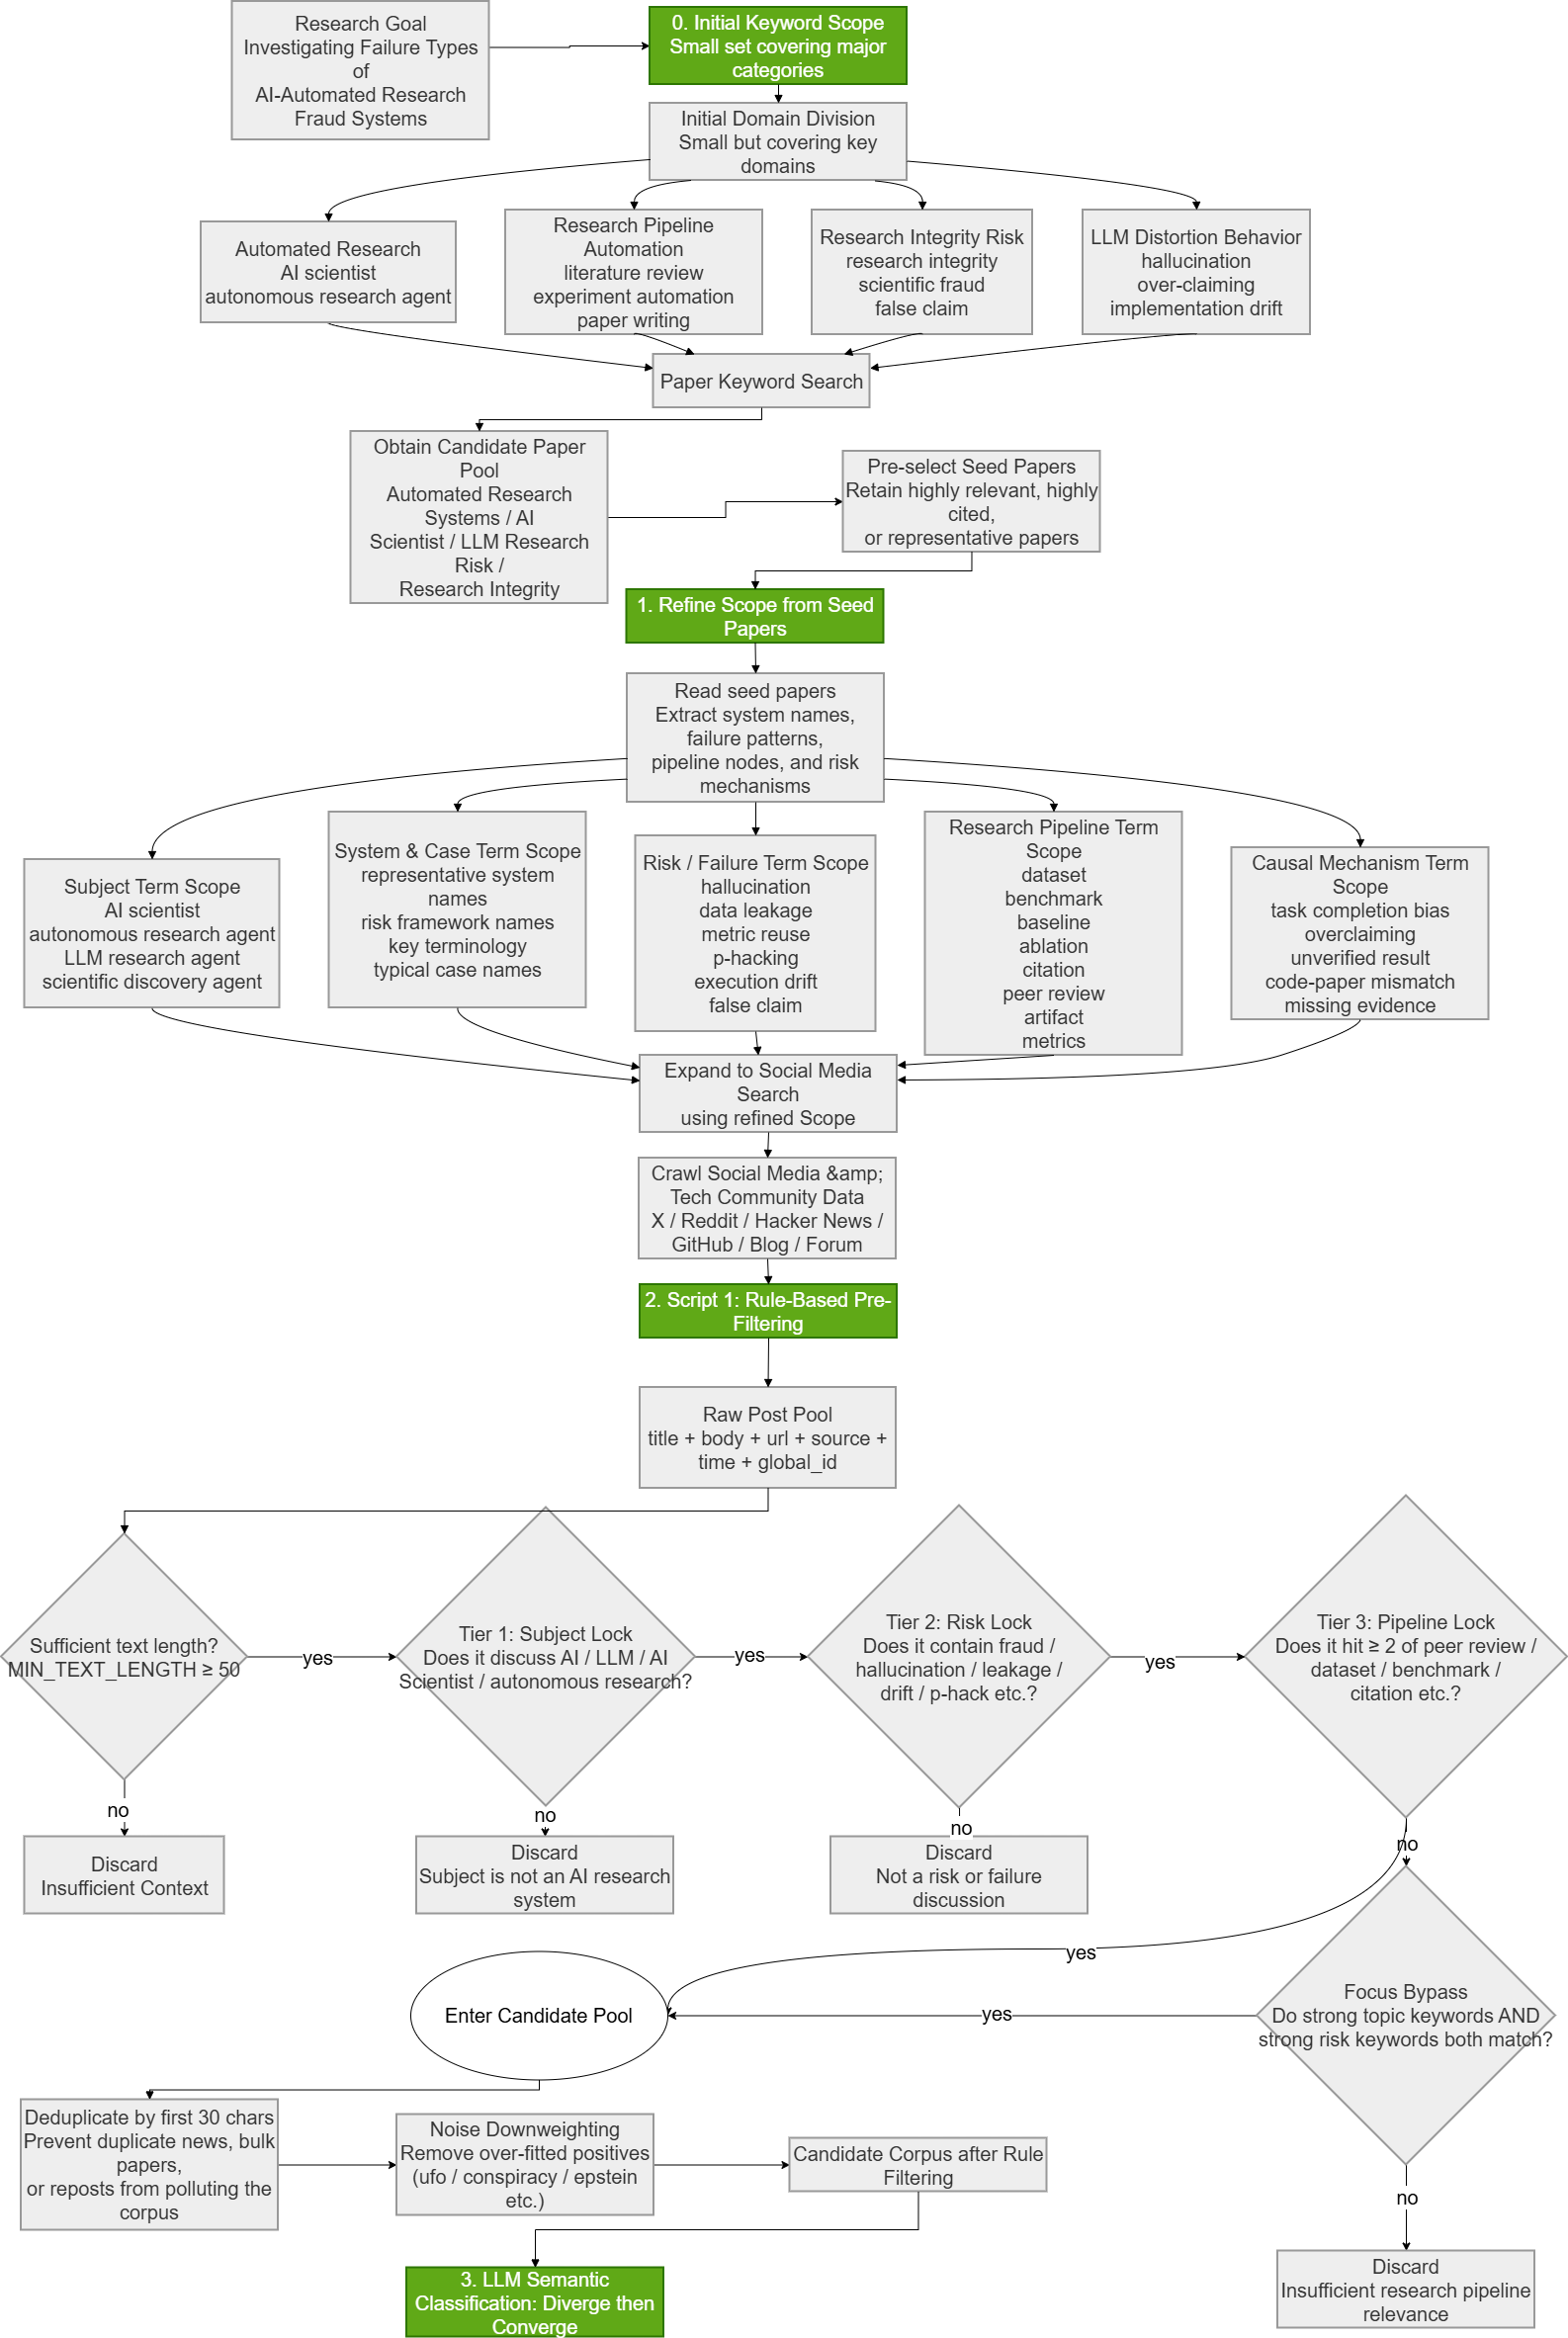
\includegraphics[width=\linewidth]{figure/fullpipeline1.png}
    \caption{Full taxonomy construction pipeline (Part 1):
    corpus construction and rule-based filtering.}
    \label{fig:fullpipeline1}
\end{figure}

\begin{figure}[!htbp]
    \centering
    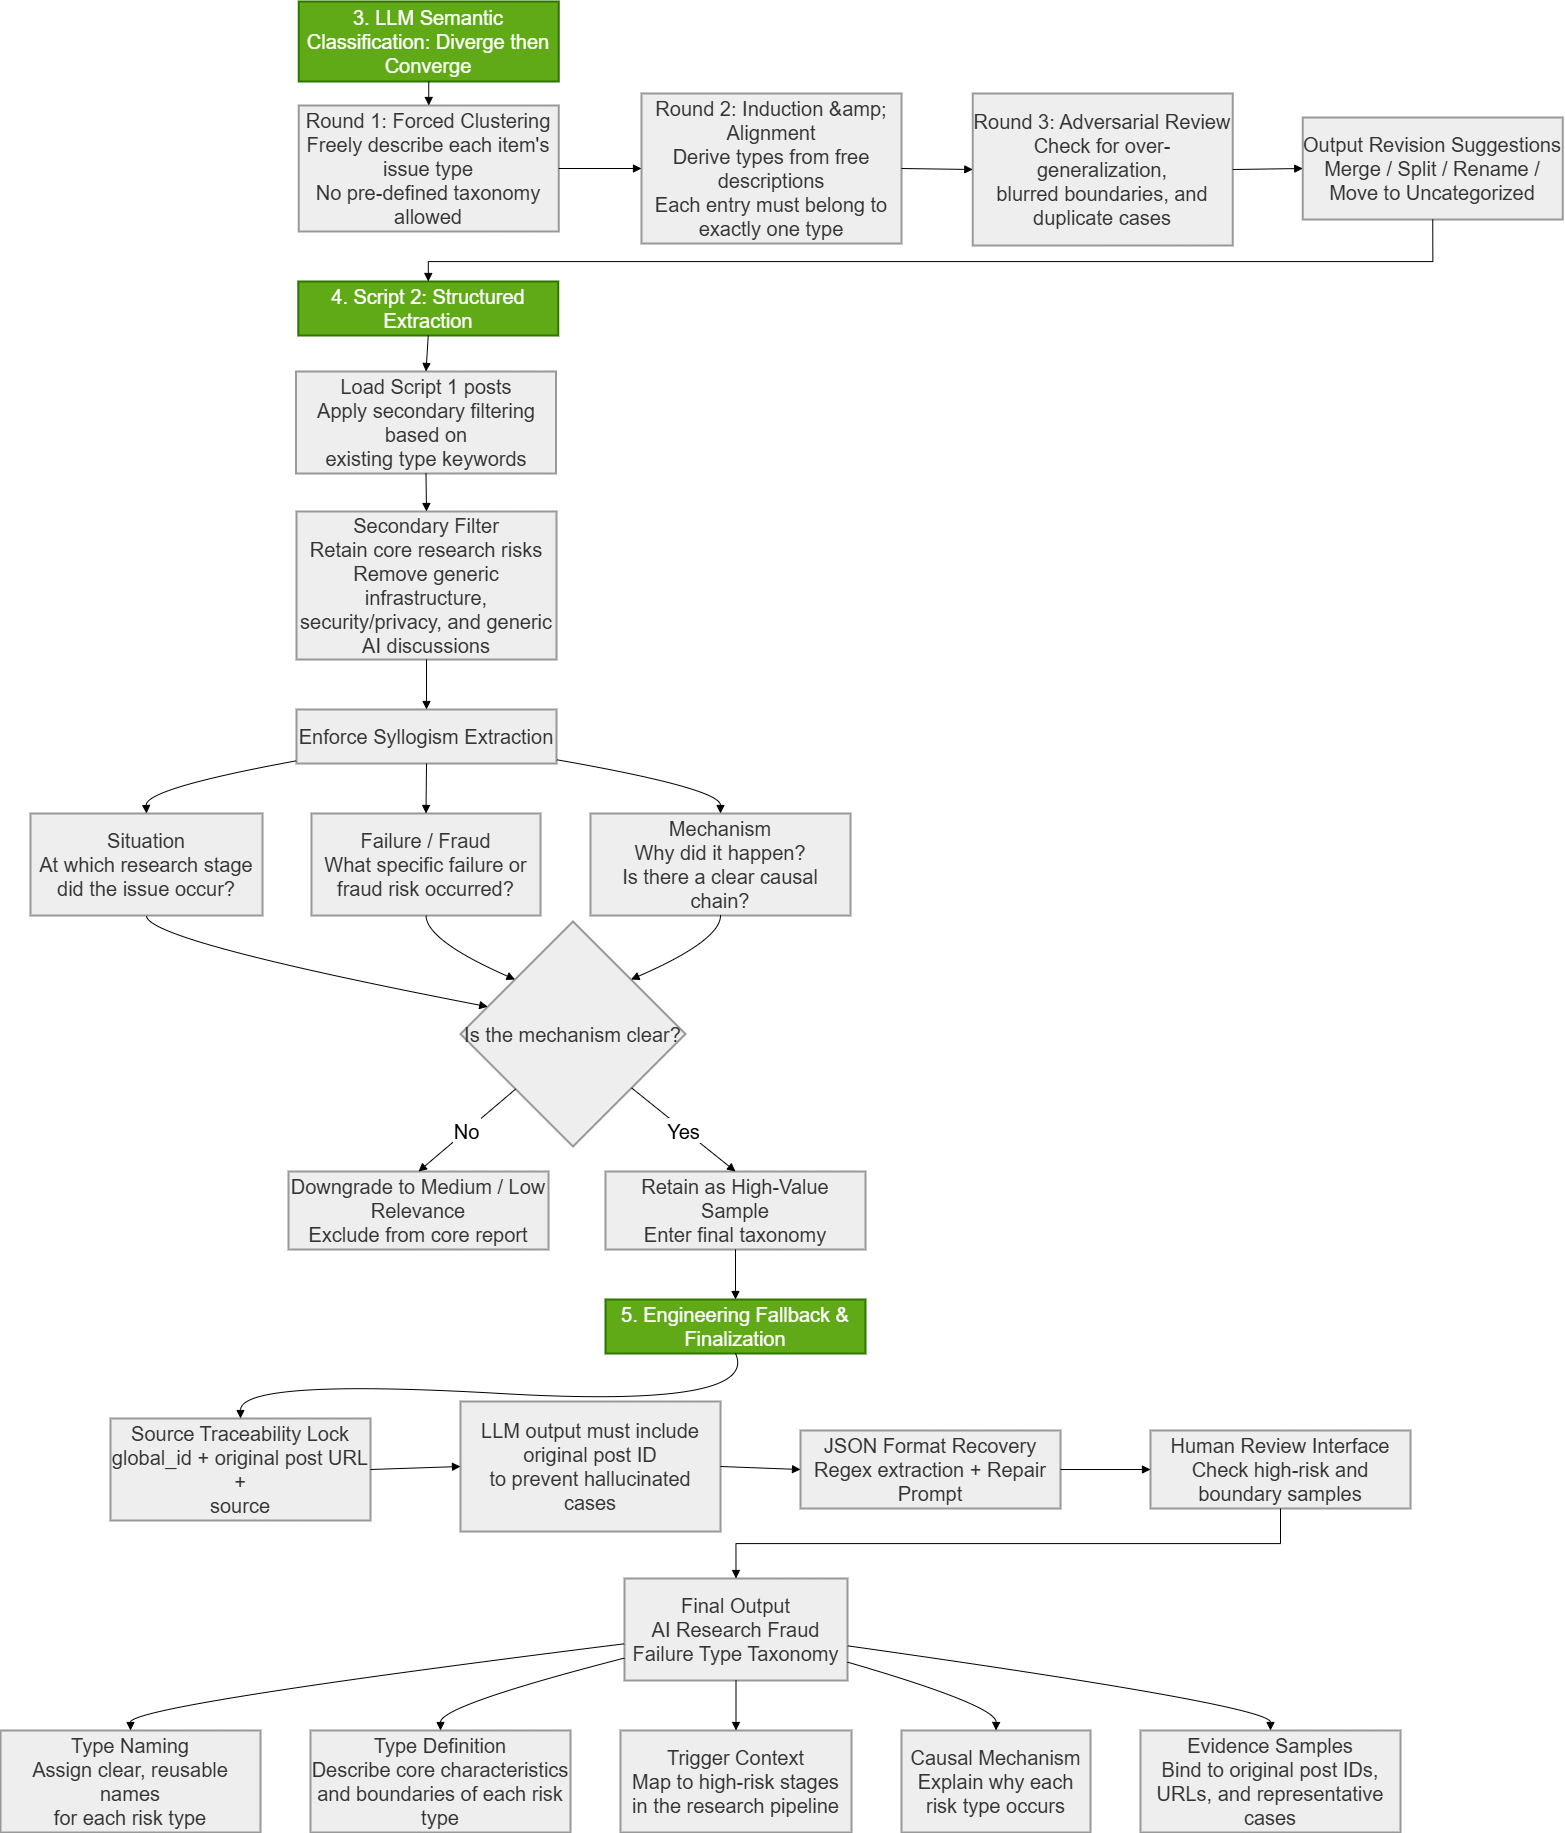
\includegraphics[width=\linewidth]{figure/fullpipeline2.png}
    \caption{Full taxonomy construction pipeline (Part 2):
    LLM semantic clustering, causal verification, and finalization.}
    \label{fig:fullpipeline2}
\end{figure}

\paragraph{Stage 1: Corpus Construction.}
Starting from broad keywords on AI research agents, automated
scientific discovery, LLM-based research workflows, research
integrity, benchmark evaluation, and data leakage, we retrieved
seed papers, expanded the search scope, and built relevance
filters for social media discussions. We crawled Reddit and
Hacker News, examining 3,556 records in total: 1,956 from
Hacker News and 1,600 from Reddit.

\paragraph{Stage 2: Rule Filtering.}
After duplicate removal, short-text filtering, and relevance
filtering, 195 Hacker News records and 447 Reddit records were
retained, then supplemented with academic literature,
developer-community materials, and peer-review artifacts.
After merging, deduplication, and final screening, the corpus
contained approximately 512 documents.

\paragraph{Stage 3: LLM Clustering.}
DeepSeek-V4 clustered the 512 documents by underlying failure
mechanism across three rounds: forced divergence (free
categorization without pre-defined taxonomy), convergent
consolidation (bottom-up induction into 5--15 categories),
and adversarial audit (boundary clarity review). This produced
14 candidate categories.

\paragraph{Stage 4: Causal Verification.}
We triangulated the 14 candidates against literature, GitHub
issues, technical blogs, and peer-review materials, retaining
only categories with sufficient evidence, distinct causal
mechanisms, direct relevance to AI-assisted research workflows,
and benchmark operationalizability. Three candidates were
excluded: context decay mainly tests long-context memory,
implicit-knowledge probes mainly test domain-specific knowledge,
and temporal contamination depends heavily on retrieval systems
and version control. These were treated as stress conditions
for future extensions rather than mutually exclusive misconduct
categories. This process yielded the final 11 categories.